\chapter{Proposed Method}
%TODO: START COPY-PASTE
\section{Overview}
   %input output only melodic constrins
   %flow chart
      \begin{figure*}[tp]
         \begin{center}
            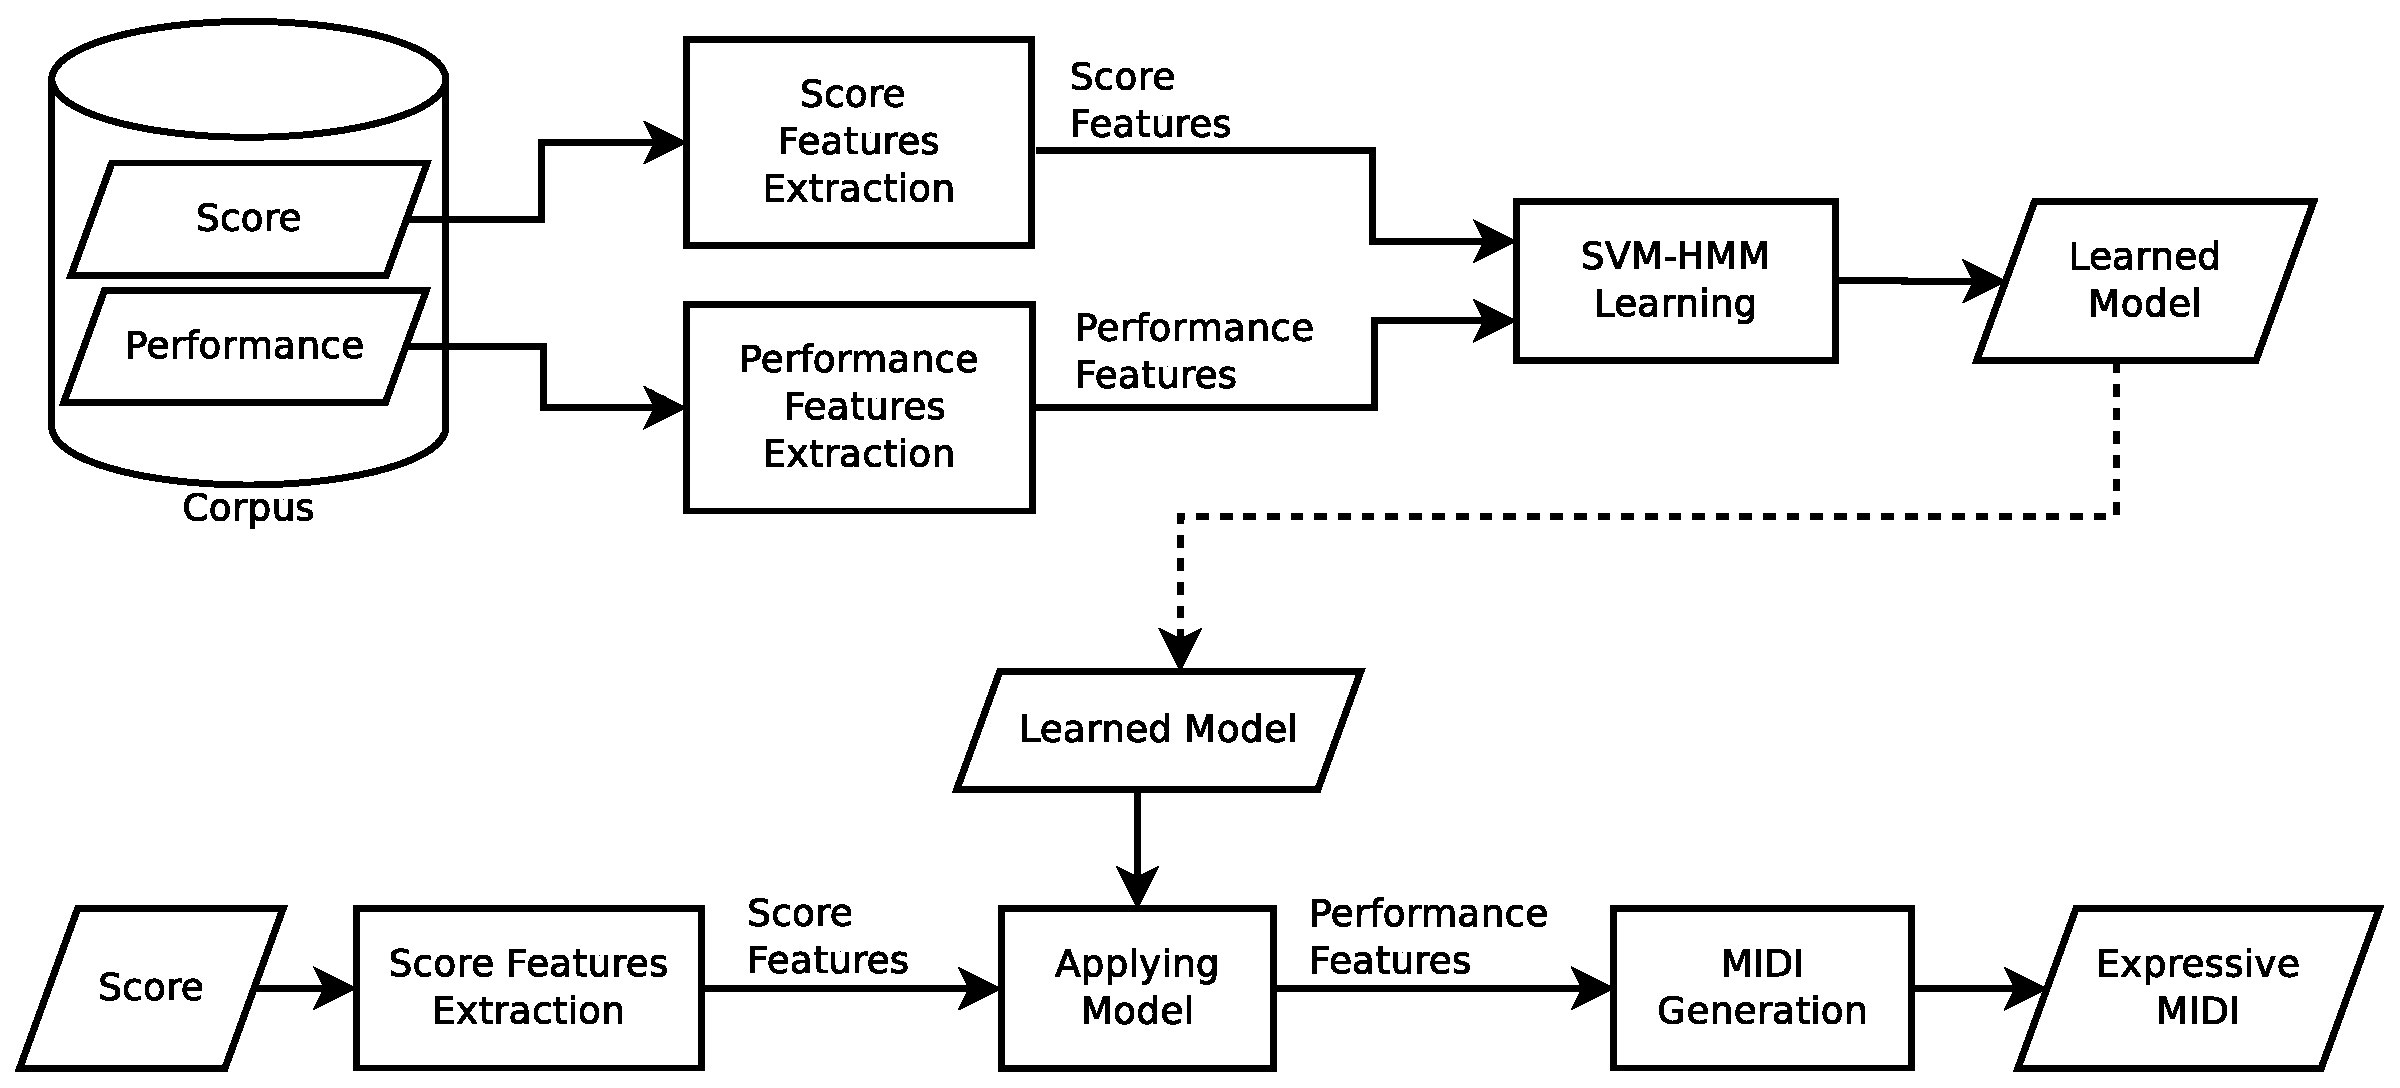
\includegraphics[width=\textwidth]{fig/sys_arch}
         \end{center}
         \caption{System Architecture} 
         \label{fig:flow}
      \end{figure*}
The high-level archtecture of the purposed system is shown in figure \ref{fig:flow}. The system is has two phases, the upper half of the figure is the learning phase, while the lower half is the generating phase.  In the training phase, score and expressive performance recording pairs are feed in, their features will be extracted and used as the input for the learning algorithm.  The learning algorithm will produce a learned model, which can be used to generate expressive performance hereafter. In the generating phase, a score is taken as input, and it's score features are extracted. The generation module ("Applying Model" box) then use the extracted features and the learned model to produce the preformance features for the score. The performance features can be viewed as the instruction for expression. With these features, an expressive MIDI performance for the input score can easily be generated.  
%TODO: refer to feature exction and corpus chapter

The system is not intend to add fixed expression to all pieces. Rather it is intended to perform music according to the style which the user wants. This kind of user interactivity can be achieved in two ways: first, the user can choose the training dataset. The dataset is organized by tags, example of tags are like performer, mood, emotion, genre, style, etc. So the user can select a subset of training sample by selecting tags. Second, the phrasing is given by the user. Since phrasing controls the overall structural interpretation of a music piece, and form a breathing feeling in music, user is given direct control over the performance.

There are still some constrains for the system now. The scores must be monophonic and contains only one musical phrase. One has to manully label the phrasing for any scores used. The learning algorith, namely structural suppor vector machine, can only perform offline learning, so the learning phase can only work in a non-realtime scenario. The generating phase can work much faster though, it can procude expressive music almost instantely after loading the score. All the scores are loaded in batch, the systme currently don't accept streaming input.

\framebox{TODO:Talk about how this chapters is layed out}

   \section{Features}
   The system is trying to mimic the process of human performance: the musican reads the explict and implict cues from the score and transform them into musical expressions. So the features can be categorized into two category: score features and performance features.  Score features are information contained in the score. Performance features corresponds to the musical expression. The basic time unit for both features are a note. 
      \subsection{Score Features}
      Score features includes:
      \begin{description}
         \item [Relative position in a phrase:]
            The relative position of a note in the phrase. From 0\% to 100\%. This feature can catch the musical hint of the opening and closing of a phrase.  
         \item [Relative pitch:]
            The pitch (in semitone) of a note relative to the pitch range of the phrase. For a phrase of $n$ notes with pitch $P_1, P_2, \dots, P_n$, $$RP = \frac{P_i -min(P_1, P_2, \dots, P_n) }{max(P_1, P_2, \dots, P_n)-min(P_1, P_2, \dots, P_n) }$$  Where $P_i$ is the pitch of note at position $t$

         \item [Interval from the previous note:] The direction of melody movement. Measured in semitone. $$IP = P_{i} - P_{i-1} $$ See figure \ref{fig:interval} for example.
         \item [Interval to the next note:] The direction of melody movement. $$IN = P_{i+1} - P_i$$ See figure \ref{fig:interval} for example.
         
      \begin{figure}[tp]
         \begin{center}
            \includegraphics[width=0.4\textwidth]{fig/interval_arrow}
         \end{center}
         \caption{Interval from/to neighbor notes}
         \label{fig:interval}
      \end{figure}

         
         \item [Note duration:] The duration of a note in beats.
         \item [Relative Duration with the previous note:] The duration of a note divided by the duration of its previous note. For a phrase of $n$ notes with duration $D_1, D_2, \dots, D_n$, $$RDP = \frac{D_i}{D_{i-1}} $$ See figure \ref{fig:duration} for example.
         \item [Relative duration with the next note:] The duration of a note divided by duration of its next note. $$RDN = \frac{D_i}{D_{i+1}} $$ See figure \ref{fig:duration} for example.

      \begin{figure}[tp]
         \begin{center}
            \includegraphics[width=0.4\textwidth]{fig/duration}
         \end{center}
         \caption{Duration from/to neighbor notes}
         \label{fig:duration}
      \end{figure}
   \item [Metric position:] The position of a note in a measure, measured by the beat unit defined by the time signature. For example, a $^4_4$ time signature will have a beat unit of a quarter note. So if the measure consists of four quarter notes, each of them will have metric position of 1, 2, 3 and 4. See figure \ref{fig:metrical}.

   \begin{figure}[tp]
      \begin{center}
         \includegraphics[width=0.4\textwidth]{fig/metrical}
      \end{center}
      \caption{Metric position}
      \label{fig:metrical}
   \end{figure}
      \end{description}

      %TODO: link to narmour group
   \begin{figure*}[tp]
      \begin{center}
         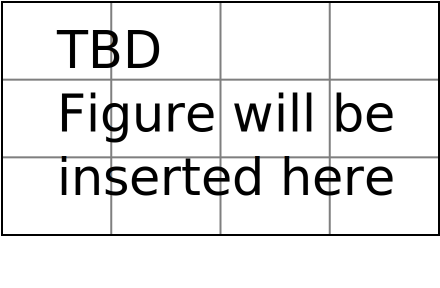
\includegraphics[width=0.8\textwidth]{fig/TBDFigure}
      \end{center}
      \caption{Example Score Features}
      \label{fig:expScoreFeat}
   \end{figure*}
      \subsection{Performance Features}
      Performance features includes:
      \begin{description}
         \item [Relative onset time bias:] 
            The onset time of a recording will not be exactly as the ones indicated on the score. Given a fixed tempo (beats/second), the score timing of each note can be calculated as tempo $\times$ (beats from the start of phrase)  . The relative onset time bias is the difference of onset timing between the performance and the score, divided by the total length of the phrase. Namely,
            $$ ROB = \frac{O_i^{perf} - O_i^{score}  }{length(phrase)}$$ Where $O_i^{perf}$ is the onset time of note $i$ in the performance, $O_i^{score}$ is the onset time of note $i$ in the score. 
         \item [Relative loudness:] The loudness of a note divided by the maximum loudness in the phrase. Measured by MIDI velocity level.
            $$ RL = \frac{L_i}{max(L_1, L_2, \dots, L_n)}$$

         \item [Relative duration:]
            The actual duration of note divided by the total length of the phrase.
            $$ RD = \frac{ D_i^{perf}}{length(phrase)}$$
      \end{description}

\begin{figure*}[tp]
   \begin{center}
      %TODO:Figure:Example JSON code
      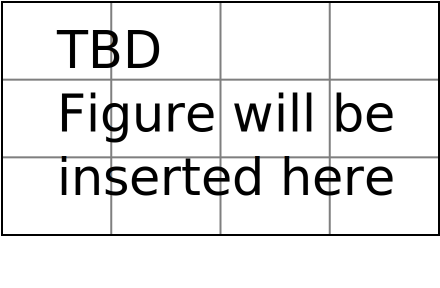
\includegraphics[width=\textwidth]{fig/TBDFigure}

   \end{center}
   \caption{Example Performance Features}
   \label{fig:expPerfFeat}
\end{figure*}
   % \section{Melodic Similarity and Sample Selection}
   % Once a score is given to the system for playing, all the samples in the database will be ranked by the melodic similarity with the given score. Here we use the melodic distance function provided by the MIDI Toolbox\cite{Eerola2004}, which is defined as follows: 
   % \begin{enumerate}
   %    \item Melodic contour is calculated by connecting each note's pitch, forming a piece-wise linear contour.
   %    \item Subtract the contour by it's mean to preserve only the relative part.
   %    \item If the two phrases has different length, re-sample both phrases with fixed intervals so both of the phrase will have contour vector of the same length.
   %    \item The L1 norm (a.k.a Taxicab distance) of these two contour vector is the similarity measure. 
   % \end{enumerate}
   % The reason I choose melodic contour is because it yields best results in finding melodic similarity, which is shown in \cite{Hoffmann-engl2005}.

      %TODO: not included features: e.g. notation

   \begin{figure}[tp]
      \begin{center}
         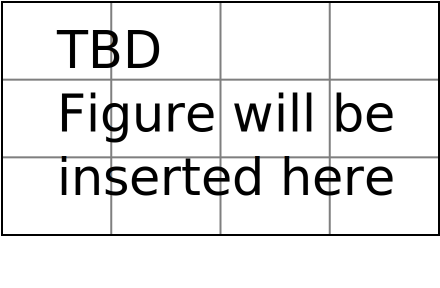
\includegraphics[width=0.8\textwidth]{fig/TBDFigure}
      \end{center}
      \caption{Example Performance Features}
      \label{fig:expPerfFeat}
   \end{figure}
   \subsection{Normalizing Onset Timing}
\begin{figure}[tp]
   \begin{center}
      %TODO:Figure:Normalization Schemes
      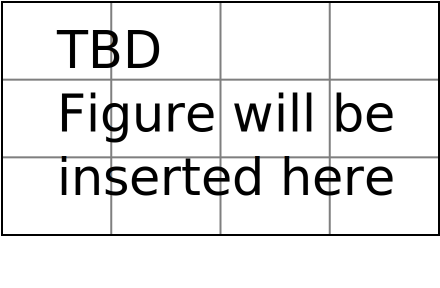
\includegraphics[width=\textwidth]{fig/TBDFigure}

   \end{center}
   \caption{Normalization Schemes}
   \label{fig:normalization}
\end{figure}
   The relative onset timing bias feature must be normalized to get meaningful result. For example, a phrase is played very fast by the performer, say, the played length is only 70\% of the notation. If the first note is aligned, the onset timing bias will grow linearly until the end of the phrase, the last note will have a onset timing bias of about 30\% of the phrase. But from the definition of this feature, the timing bias should be roughly less than half of  a note's length, and it's mean should be around zero. This 30\% value will introduce a relative large value in the training corpus, and thus there may be very large output value from the generation phase. If the model predict that a note should be played early or later for 30\% of the phrase length, the melody will be messed up. 

   There are four possible type of normalization: the first note can either be aligned at onset, or not aligned at all. The last note can be aligned at onset, or aligned at note off event.  The incentive for not aligning the first note is that the performer may intend to use an early start or delayed start as an expression, if the first note is aligned by it's onset, the first note in every phrase will have a onset timing bias feature of value zero. In other words, the early/delayed start expression is lost. %But each normalization method are equally reasonable theoretically, so we need to use empirical data to verify them. The experiment is explained in section \ref{TODO:experiment}. The experiment result showed that [TODO: result]
   But experiments shows that none of these methods can fit all training samples. One may get good result by using one method on part of the corpus, but may result in large bias when applying it to the rest of the corpus. Since none of the methods can fit all, we take a different approach: let the program find the best fitting ratio for normalization. To achieve this goal, we first have to define how "fit" two phrases are, or how to define the distance between phrase. If the onset time of all the notes in a phrase are concatenated into a vector, the $l^2$-norm of the tow vectors can be treated as the distance. Note that the two vectors must have the same size, because the recordings are required to match note-to-note with the score. So the problem becomes how to find a optimal scaling ratio such that the scaled recording has the minimum distance from the score. The Brent's method\cite{TODO:brent1973} is used to find the optimal ratio. To speed up the optimization and prevent extreme values, we imposed a range of $[initial_guess \times 0.5 , initial_guess \times 2]$ to the optimizer. The $initial_guess$ is used as a rough estimate of the ratio, calculated by aligning the first and last onset of the phrase. Than we assume the actual ratio will not be smaller than half of $initial_guess$ and not larger than twice of $initial_guess$. The two numbers 0.5 and 2 are arbitrary chosen, but most of the empirical data suggest is valid most of the time. 
   \framebox{TODO: conclusion}


   %TODO:Automatic onset timing normalization
   %TODO:Define the distance
   %TODO:SciPy optimization method


      %TODO: 4 onset diffs
   \section{Learning Phase}
   In the learning phase, the features extracted in the previous stage is feed into a machine learning algorithm to produce a phrase model. The learning module has a input/output interface that is independent of the underlying algorithm, so different algorithm can be implemented without changing the overall structure of the system.

%TODO: sample loader
   A training sample is loaded with the sample loader module, since a training sample is consisted of a score and a recording, the sample loader finds the two files given the sample name, and load them into \texttt{music21.Stream} object. The music21 library will convert the musicXML and MIDI format into a python Object hierarchy that is easy to access and manipulate by python code. The loaded score are then handed to the feature extractor module.

   In  order to keep the system architecture simple, the feature extractors should be as independent as possible, so the features can add or remove individual feature without breaking the system, and the features can be extracted in parallel. To achieve this, each feature must implement a common feature extractor interface, and feature extractors can't communicate with each other. 

   But sometimes a feature is based on other features, for example, the "relative duration with the previous note" is calculated based on the "duration" feature. But since they can't share informations, the "relative duration" feature extractor must call the "duration" feature extractor during its execution. To avoid redundant calling of feature extractors, we implemented a caching mechanism. Say, the "duration" feature had been extracted for a training sample, it's value will be cached during this execution session; when the "relative duration" extractor calls the "duration" extractor again, the value is retrieved from cache without re-calculation.  This method can speed up the execution while keeping the system complexity low.

   The the extracted features are aggregated into a json file, which will serve as the input for the learning algorithm. Each sample contains the extracted score and performance features. The learning algorithm can then do any pre-processing on the features, such as aggregation or quantization. The output of this module is the algorithm specific model description. For example, a linear regression algorithm will output the regression parameters. The algorithm is required to produce a model file containing the model description, but the system doesn't care about the internal format of the model description file, it will simply feed this model file to the generation module in the generation stage. So the developer of the learning module has to implement methods to write and read the model file themselves.

   In the early stage of this research, linear regression is used. The results of linear regression is shown in \cite{Lyu2012}. In this thesis, Structural Support Vector Machine\cite{Joachims2009} is used instead. The detail of Structural SVM will be in the next Chapter.
   %TODO: SVM-HMM
   \section{Generating Phase}
      After the model for a input phrase is generated, we can than use the score features and model coefficients to calculated the performance parameters. These performance parameters will then be applied to the input score.
      
      %TODO: no post-processing now
      %TODO: scaleable post-processing?
      Some post-processing will be made for each performance parameters: The first time bias will be reduced if it is too negative and create a negative onset time for the first note. Loudness will be shift and shrink to a predefined range. The default is 80~127 MIDI loudness level. This will ensure the loudness in the output will be in acceptable range. 
      
 So after we input an input score, its score features will be extracted. These score features combined with regression model will be used to calculate performance features. The result will be an expressive MIDI output. Ready to be played by hardware or software synthesizer.  
 \framebox{TODO:off-line vs on-line}
 \framebox{TODO:Discuss timber and instrument specific techniques}
 \framebox{TODO:Discuss timber and instrument specific techniques}
   
%TODO:END COPY-PASTE
